\documentclass[12pt, notitlepage]{article}
\usepackage[utf8]{inputenc}
\usepackage{multicol}
\usepackage{multirow}
\usepackage[margin=0.5in]{geometry}
\usepackage[utf8]{inputenc}
\usepackage{tikz}
\usepackage{graphicx}
\graphicspath{{./images/}}
\usepackage{soul}
\usepackage{listings}
\usepackage{xcolor}
\usetikzlibrary{arrows}
\usepackage{mathtools}
\usepackage{amsmath}
\usepackage{pgfplots}
\pgfplotsset{compat=1.8}
\usepgfplotslibrary{statistics}
\usepackage{float}
\usepackage{tabto}
\usepackage{caption}

\title{CSE 145 - Final Project}
\author{Daniel Xiong (dxiong5@ucsc.edu)\\
		Nyi Nyi "Scott" Zin (nzin@ucsc.edu)}
\date{Due June 7}

\begin{document}
\maketitle
\section{Introduction}
The goal of our final project was to try and find out if there was a correlation between Elon Musk's twitter account and his stock \$TSLA. To do this, we web scrapped all of Elon's tweets from June 28 2010, the day \$TSLA IPO was opened until 5/26/2020, the day we initially web scrapped the data. To do this, we first made some visualizations to try and get a better understanding of our data. We then ran a sentiment analysis on Elon's tweets and then correlated those to the closing of the market days to see if there was a correlation. We then used multiple models such as a neural net, naive bayes, decision tree, and random forest to predict whether or not Elon's tweets had an effect over the \$TLSA stock.
\section{Tools Used}
This assignment was completed using Python 3.7 (sklearn, keras, pandas, matplotlib). Refer to the
README to find instructions on how to run the code.
\section{Data Pre-processing}
Our spreadsheet of tweets sometimes had non-English characters so we decided to delete all the rows with that. We also deleted mentions within a tweet because we believed that it would have no effect on the sentiment analysis. The tweets also sometimes were only pictures without any text so we deleted those entries as well. 
\section{Data Understanding and Analysis}
To get a better understanding of the data we were dealing with, we decided to make visuals out of them such as the amount of tweets per year since 2010, a distribution of the results from the sentiment analysis, and to compare the stock price of \$TSLA and the sentiment analysis, we chose to pick an arbitrary month in which we showed the changes in sentiment and the changes in stock price.\\
The first two figures are a simple bar graph showing the amounts of time Elon Musk tweeted within a year and the second figure is just a distribution of what our sentiment analysis returned. \texttt{figure 3} required a little more work in which we had to determine dates where the market was closed and push tweets back such that if they were on a day the market was closed or was tweeted after it closed for the day, it would contribute towards the next day. After doing this, we needed to take the sentiments of those graphs and average them out so that they aligned with a stock day. \texttt{figure 4} is just another graph of how the closing price of \$TSLA changed over the time of a month in 2017.
\begin{figure}[h!]
	\centering
	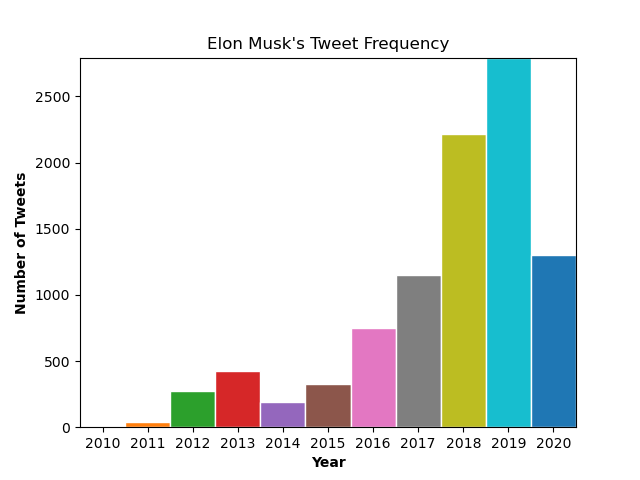
\includegraphics[scale=0.8]{images/Frequency.png}
	\caption{Frequency of tweets per Year}
	\label{fig:F}
\end{figure}
\begin{figure}[h!]
	\centering
	\includegraphics[scale=0.8]{images/sentiment_distribution.png}
	\caption{Sentiment Distribution}
	\label{fig:SD}
\end{figure}
\begin{figure}[h!]
	\centering
	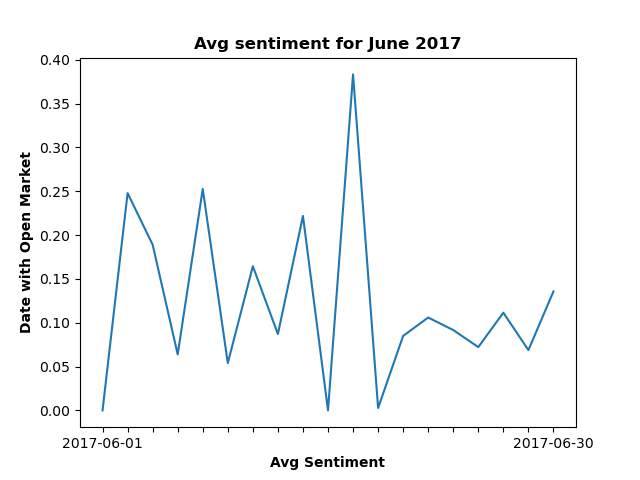
\includegraphics[scale=0.8]{images/sentiment_overtime.png}
	\caption{Sentiment distribution for June 2017}
	\label{fig:SO}
\end{figure}
\begin{figure}[h!]
	\centering
	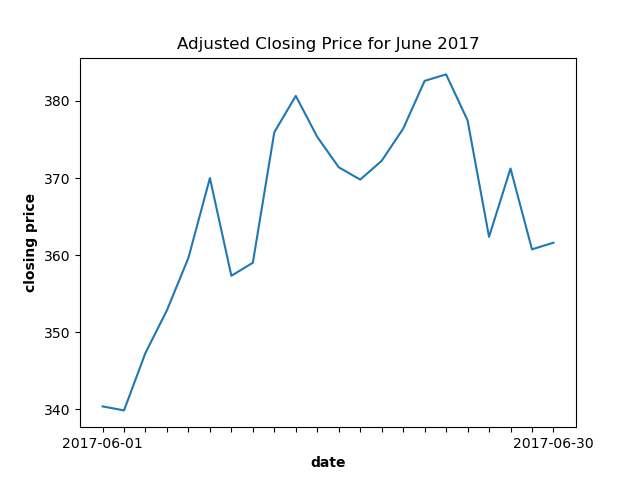
\includegraphics[scale=0.8]{images/stock_overtime.png}
	\caption{Stock Price for June 2017}
	\label{fig:SP}
\end{figure}
\clearpage
\pagebreak

\section{Prediction Model}

\section{Conclusion}
\end{document}